\documentclass[10pt,a4paper,twoside]{tudelft-report}
\usepackage[noabbrev]{cleveref}
\crefname{lstlisting}{listing}{listings}
\Crefname{lstlisting}{Listing}{Listings}
\usepackage{todonotes}
\presetkeys{todonotes}{inline, noline}{}
\usepackage{subcaption}
\usepackage{enumitem}
\usepackage{listings}
\usepackage{hhline}
\usepackage{proof}
\usepackage{natbib}
\usepackage{changes}
\usepackage{wrapfig}
\usepackage{url}
\usepackage{verbatim}
\usepackage{bbding}
\usepackage{booktabs}
\usepackage{float}
\usepackage{tabularx}
\usepackage{threeparttable}
\usepackage{usebib} % Use data defined in the bib file.
\usepackage[justification=centering]{caption}
\bibinput{references}

\graphicspath{{images/}}

% \usepackage{todonotes}
\usepackage{xifthen}
% \usepackage[usenames,dvipsnames,svgnames,table]{xcolor}
\usepackage{titlesec}
\usepackage{ulem}
\newif\ifcomments

% % Disable comments by commenting the line below this one
\commentstrue

\ifcomments
% TODO's
%   \newcommand{\todo}[1]{{\color{red} TODO: #1}}
  \newcommand{\todolater}[1]{\textbf{*}}

  % maybe
  \newcommand{\maybe}[1]{{\itshape\color{orange}\{ {#1}\}}}
  \newcommand{\maybex}[1]{{\color{orange}({#1})}}

  \newcommand{\replace}[2]{{\color{red}\sout{#1}}{\color{green}#2}}
\else
  \newcommand{\todo}[1][SOMETHING]{}
  \newcommand{\todolater}[1]{}
  
  \newcommand{\maybe}[1]{}
  \newcommand{\maybex}[1]{}
  
  \newcommand{\replace}[2]{#2}
\fi

\usefont{T1}{cmr}{m}{n}

\definecolor{commentgray}{RGB}{169,173,178}
\definecolor{stringblue}{RGB}{2,48,96}
\definecolor{keywordred}{RGB}{213,60,76}
\definecolor{codedefault}{RGB}{36,41,46}

\begin{document}

% Related Work
% Problem Analysis ("4 main parts")
%       Sub problem identification
% Requirement Analysis
% Framework and Tools
% Conclusion
% \begin{titlepage}

\newcommand{\HRule}{\rule{\linewidth}{0.5mm}}

\center
 
\textsc{\LARGE Delft University of Technology}\\[1.5cm]
\textsc{\Large Bachelor Graduation Project}\\[0.5cm]
\textsc{\large Initial Research Report}\\[0.5cm]

\HRule \\[0.4cm]
{ \huge \bfseries UrbanSearch}\\[0.4cm]
\HRule \\[1.5cm]
 

\begin{minipage}{0.4\textwidth}
\begin{flushleft} \large
\emph{Authors:}\\
Tom \textsc{Brunnik}\\
Marko \textsc{Malis}\\
Gijs \textsc{Reichert}\\
Piet \textsc{van Agtmaal}\\
\end{flushleft}
\end{minipage}
~
\begin{minipage}{0.4\textwidth}
\begin{flushright} \large
\emph{Supervisor:} \\
Claudia \textsc{Hauff}

\emph{Clients:} \\
Evert \textsc{Meijers}\\
Antoine \textsc{Peris}
\end{flushright}
\end{minipage}\\[4cm]


{\large \today}\\[3cm]

\vfill

\raggedright

\includegraphics[width=0.25\textwidth]{logo}

\end{titlepage}
% \providecommand{\keywords}[1]{\textbf{Keywords:} #1}
\begin{abstract}
It is yet to be discovered how the importance of cities in the global network can be elucidated. In this paper, we develop a methodology to be able to reveal an answer to this matter. ...\\
\keywords{urban, city, data mining, document analysis, filtering}
\end{abstract}
% \newpage
% \tableofcontents
% \newpage
% This is the user manual for the UrbanSearch Web Interface. Here we will explain the different functions of the interface and how to use them. 
% \section{Related Work}
In this section we will discuss the current methods to extract relations and their strength between cities. Currently there are only two methods that are considered. The first is to manually process data from search engines. The second is to look at in what cities companies are located. After discussing these two methods we will also take a loot at NLTK \cite{nlkt_stemming}. NLTK is  a text processing tool on which (a part of) our system will be based.\\

The first currently used method is to manually process data from search engines. Researchers will input a query in a search engine (for example Google). Then they will check how many websites are found. They will also take a tiny subset of those websites, and classify them manually. There are a few problems that arise with this method. The first one is that a lot of works needs to be done by hand, which takes a lot of man-hours more then when it is done by a machine. The second is that humans are biased on what they belief is important instead of when it is automatically generated. \\

Another method that might be used is to look at companies and look at in what cities they are located. Although this might be a good indicator of the economic relations between cities, this completely ignores other relations cities might have with each other.\\

With our method we would like to process the websites through an algorithm by using the raw text from this. NLTK is a program to find relations between texts. Therefor we might base our own application on it. We would need to extend it so that we can use data from websites and so that we can visually show the data. Also although NLTK can find relations between text there are some algorithms which NLTK does not use and we might consider.

\begin{comment}
In economics there is the question "What factors play a role in economic growth?". To answer this question you would first need to give a clear definition of economic growth itself. Economic growth can be seen as a positive change in the level of goods and services produced by a city over a certain period of time. An important characteristic is that economic growth is not the same in different sectors. Economic growth can be achieved when the rate of increase in total output is greater than the rate of increase in population of a city. \\

According to Harvard University three general theories of Economic Growth within cities \cite{glaeser1992growth} are those of Marshall-Arrow-Romer (MAR) theory (1986), Porter's theory (1990) and Jacobs theory (1969). These theories focus on knowledge spillovers and claim they are most effective in cities because communication between people is more extensive. The thoeries are based on in one company improves techniquely other companies near it will also benefit. These theories differ on whether monopolies or competition benifit the growth and whether the influence is within the same industry or not (e.g. brassiere and lingerie industry). \\
Other studies focus instead on the growth of countries instead of cities. Economist Alexander Cairncross wrote that the most important factors are investment, technical process, development and trade \cite{cairncross2013factors}. Economist Stanley Fischer focusses on the influence of macroeconomics (inflation, large budged deficits, distorted foreign echange markets) \cite{fischer1993role}. Economists Rudiger Dornbusch and Alejandro Reynoso claim the most important aspects differ per region \cite{dornbusch1989financial}. \\
In other words, there are many theories and there is much research on what plays an important factor in economic growth. Although MAR's Porter's and Jacob's theory do claim one of the reason for more economic growth in cities is due to more communication between people, much research into the connectivity between cities seem to be missing. One approach that has been taken is to look at where international companies are located. This only gives limited information however. Therefore we would like to see what information can be gathered from the internet by using search engines with input consisting of 2 cities.
\end{comment}  
% \section {Requirements}

\subsection {Must haves}

\begin{enumerate}
    \item{General} 
    \begin{enumerate}
        \item Adding city names
        \item Grouping relations and “zooming” on these relations
    \end{enumerate}
    
    \item{Search Engine} 
    \begin{enumerate}
        \item Filter results
        \item Data mining
    \end{enumerate}
    
    \item{Filtering} 
    \begin{enumerate}
        \item Logic Filters 
        \item Relations Filters
    \end{enumerate}
    
    \item{Machine Learning} 
    \begin{enumerate}
        \item Types of relations
    \end{enumerate}
    
    \item{Visualization}
    \begin{enumerate}
        \item Statistics of relations? Query relations
        \item Strength of relations
        \item Types: ML CBS defined
    \end{enumerate}
\end{enumerate}


\subsection {Should haves}

\begin{enumerate}
    \item{General}
    \begin{enumerate}
        \item Pluggable datasets
    \end{enumerate}
    
    \item{Machine Learning}  
    \begin{enumerate}
        \item Generalising relations, grouping relations
    \end{enumerate}
\end{enumerate}


\subsection {Could haves}

\begin{enumerate}
    \item{General}
    \begin{enumerate}
        \item International city names
    \end{enumerate}
    
    \item{Visualization}    
    \begin{enumerate}
        \item Front end for the app
    \end{enumerate}
\end{enumerate}

\subsection {Would haves}
% \section{Frameworks and Tools}

\subsection{Extraction}
\subsubsection{Information Sources}

\paragraph{Common Crawl}
Common Crawl \cite{commoncrawl} is a freely accessible corpus of the pages across the web. Their data is updated and released on a monthly basis. Many researchers have used the data for varying purposes~\cite{smith2013dirt}~\cite{muhleisen2012web}~\cite{singh2012wikilinks}. Since the UrbanSearch project requires us to crawl the web (see section {\color{Red} FIXME}), the corpus is a very suitable candidate for us to work with.

The data of Common Crawl comes in three formats: 
\begin{itemize}
\item[WARC]
\item[WAT]
\item[WET]
\end{itemize}

For extracting data from Common Crawl, many open-source libraries are available. Common Crawls' official website refers to \texttt{cdx-index-client}\footnote{https://github.com/ikreymer/cdx-index-client} as a command line interface to their data. It allows for, among others, specifying which index to use, supports multiple output formats (plain text, \texttt{gzip} or \texttt{JSON}) and can run in parallel.

\paragraph{Eurostat}
{\color{Red} FIXME @Gijs: niet iets zeggen over wat het is?}
We identified Eurostat as a source that is not useful for the problem we're going to solve. Although Eurostat contains a lot of statistics on European cities, there is not enough useful information which contributes to giving more insight into the network connectivity of cities. Therefore, we did not include Eurostat as an information source.
\subsubsection{methods}

\subsection{Filtering and Categorizing}

\subsubsection{Clustering}
\subsubsection{Filtering}
\subsubsection{Machine Learning}
\subsubsection{TF-IDF}
basic idea: 1. using training data to assign values on words - filter meaningless words - assign words with highest value as categories? 2. Do the same on training data for each category (choose a few documents manually per category) and then check for websites for which categories has the highest value.

\subsection{Search Queries}

\subsubsection{Enter Queries}
\subsubsection{Get Results}
\subsubsection{Specifications}

\subsection{Visualisation}
\subsubsection{neo4j?}

\subsubsection{Connection between cities}
\subsubsection{The Strength of these connections}
% \newpage

\section{Code Quality}
To ensure code quality in our project we used several methods. The results from SIG \cite{sig}, a tool to ensure code quality and maintainability, are discussed and the testing is discussed.

\subsection{SIG \& BetterCodeHub}
SIG, Software Improvement Group, gives detailed insight needed to achieve better code quality and maintainability. SIG rates the code on a five star scale based on nine different values concerning code quality. Before submitting code to SIG we used BetterCodeHub\cite{better_code_hub} to check for possible faults in our code. BetterCodeHub does partly what SIG also does, but it is done online instead and can be done on every moment. Code was submitted to SIG on week 5 and week 9 of the project. Feedback can be found in appendix \ref{sig_fb}.

\subsubsection{week 5}
The first feedback from SIG was in the fifth week of development. Before uploading on BetterCodeHub our code passed all checks. For SIG it had a score from four out of five stars which means our code is above average maintainable. The last star was missed because the code is above average complex. This means that some of the functionality of some methods should be split into separate methods.
\todo{fixed this?}

\subsubsection{week 9}


\subsection{Testing}
We tested the program using three different testing methods. The first is unit testing, which tests the separate components individually. Selenium testing for testing the front-end of the app. And system testing for testing the different components together.


\subsubsection{Unit Testing}
Unit testing is done by writing automatic tests and making sure they pass every time the tests are executed. Unit tests test each method of a function separately, checking that the method does what it is supposed to do. If the method would need information from outside the class that information is mocked. This means that instead of using that other class, a fake object is made which returns a fake value. This ensures the tests will never fail due to changes in other classes. In total these test cover \todo \% of the code.

\paragraph{Selenium}
Selenium tests are automated tests that are run to test the front-end of systems. Just as normal unit testing, selenium testing is useful for regression testing.

\subsubsection{Integration tests}
Integration testing uses automated tests which test how well different components of the system work together. This is done more or less the same as unit testing, however whilst you would mock methods from other classes in unit testing, with integration testing you do not. It is assumed that the separate modules are unit tested, therefor if an error occurs it is because something is wrong with the interaction between the modules and not with the modules themselves. 

\subsubsection{System Testing}
Last we are also using system testing. System testing provides a more complete test of the entire system. This means it is useful to detect faults in the overall system, but less easy to determine where these faults may be located. System testing is done manually, which means the tests can not be easily repeated when the system changes whilst with other testing techniques this is possible. 

\subsubsection{Acceptance Testing}

% \chapter{Validation}

\section {machine learning}
To test the machine learning we will manually search for a small set of 50 pages per class. We will then manually decide to which class we would expect those pages to be sorted. Then we will run the algorithm and check whether or not a page was correctly sorted. There are 4 outcomes per page per class: true/false positives and true/false negatives. Positives are the pages that should be sorted to that class; true means they were sorted to that class, false meaning they were not sorted to that class. Negatives are pages that should not be sorted to that class and in this case true means they were indeed not sorted to that class and false means they were. So the true values are the ones that should be high. From this we can say how accurate our classifier is.

\section{unit tests}

\section{selenium tests}

\section{SIG}
SIG \cite{sig}, short for software improvement development group, is a tool to give deep code visibility we require so we can remedy current problems and prevent future vulnerabilities. A part of sig \todo{}(?) also includes betterCodeHub \cite{better_code_hub} which checks our code in 10 steps:
\begin{enumerate}
    \item \textbf {Write short units of code} \\
    Units of code should be no longer than 15 lines.
    \item \textbf {Write simple units of code} \\
    Separate units of code should contain no more than 4 branch points (if, for, while, etc)
    \item \textbf{Write code once} \\
    Shared code should be extracted, either to a new unit or to a super class
    \item \textbf{Keep unit interfaces small} \\
    The number of parameters per unit of code should be no more than four.
    \item \textbf{Separate concerns in modules} \\
    Identify and extract responsibilities of large modules to separate modules and hide implementation details behind interfaces.
    \item \textbf{Couple architecture components loosely} \\
    minimizing the amount of interface code (e.g. by using 'abstract factory' design pattern)
    \item \textbf{Keep architecture components balanced} \\
    Organize code in such a way that the number of components is between 2 and 12, and ensure the components are of approximately equal size (keep component size uniformity less than 0.71).
    \item \textbf{Keep your codebase small} \\
    Refactor existing code to achieve the same functionality using less volume, and prefer libraries and frameworks over "homegrown" implementations of standard functionality.
    \item \textbf{Automate tests} \\
    Add tests for existing code every time you change it.
    \item \textbf{Write clean code}\\
    Remove useless comments, commented code blocks, and dead code. Refactor poorly handled exceptions, magic constants, and poorly named units or variables.  
\end{enumerate}

\begin{comment}
- double city names
- city names with meaning (leiden)
- city/province names (utrecht / groningen / zeeland)
\end{comment}
% 
\chapter{Process}

\todo{fit this in somewhere}

\section{Collaboration between the team members}
The collebaration between the team members went well. The team members worked in a room in the faculty of architecture from 9-5 each day. Three of the four team members knew each other already. The work was devided even over the team members. 

\section{Collaboration between the team members and the TU Delft Coach}
Each week 9:30 on monday the team members had a meeting with the TU Delft coach. In the beginning there were some communication issues between the team and the coach but as the process went on communication became better.

\section{Collaboration between the team members and the client}
The collaboration between the team members and the client was good as well. 
Weekly meetings helped the team members making the productas good as possible to the clients wishes. 
% \newpage
\section{Implementation}
\todo{To do? To fake? To leave out? You decide!}

\subsection{Scrum}

\subsection{Implementation per week}

\subsubsection{week 1}
\subsubsection{week 2}
\subsubsection{week 3}
\subsubsection{week 4}
\subsubsection{week 5}
\subsubsection{week 6}
\subsubsection{week 7}
\subsubsection{week 8}
\subsubsection{week 9}

% \chapter{Conclusion}

\todo{ Start with "In the past few months we blah" and shortly mention the chapters
 Mention the project goal and how well it is met, without duplicating the 
 evaluation chapter}

\section{related work}
First, we discussed related work. We saw that there are currently two methods for analysing the relations between cities. Manually analysing search engine data is very slow and requires a lot of man-hours and looking at the different locations where businesses are located is only interesting for the economic relation and still misses a lot of data.
\\

\section{related work}
Second, we identified the requirements for a solution to the problem and discuss issues that might arise. The used the MoSCoW model to describe the importance of the different requirements. The most import must haves we found are being able to input place names, displaying a map with the connection data and being able to extract this data.
\\

\section{Requirement analysis}
Third, we developed a methodology for a framework that satisfies the requirements and tackles the issues. We decided to start by using data from Common Crawl, although we might later extend this to other data sources such as Delpher. After selecting relevant data (data which contains 2 or more city names) we store the data with Neo4j. We then use clustering and classifying machine learning to group the data. First we use this on all data to get the general groups (e.g. economy, health-care, immigration) and then we use this on the data per pair of cities to see what the important connection types for each city are. Then we link these connections to the general groups ('fish' might relate to economy.. etc). To visualise this data we use the graph Neo4j provides.

\section{Framework-and-tools}


\frontmatter

\lstdefinestyle{mystyle}{
    commentstyle=\color{commentgray},
    keywordstyle=\color{keywordred},
    numberstyle=\tiny\color{codedefault},
    stringstyle=\color{stringblue},
    basicstyle=\footnotesize\tudcffamily,
    breakatwhitespace=false,         
    breaklines=true,                 
    captionpos=b,                    
    keepspaces=true,                 
    numbers=left,                    
    numbersep=5pt,                  
    showspaces=false,                
    showstringspaces=false,
    showtabs=false,                  
    tabsize=2
}
 
\lstset{style=mystyle}
% image of UI?
\begin{titlepage}

\newcommand{\HRule}{\rule{\linewidth}{0.5mm}}

\center
 
\textsc{\LARGE Delft University of Technology}\\[1.5cm]
\textsc{\Large Bachelor Graduation Project}\\[0.5cm]
\textsc{\large Initial Research Report}\\[0.5cm]

\HRule \\[0.4cm]
{ \huge \bfseries UrbanSearch}\\[0.4cm]
\HRule \\[1.5cm]
 

\begin{minipage}{0.4\textwidth}
\begin{flushleft} \large
\emph{Authors:}\\
Tom \textsc{Brunnik}\\
Marko \textsc{Malis}\\
Gijs \textsc{Reichert}\\
Piet \textsc{van Agtmaal}\\
\end{flushleft}
\end{minipage}
~
\begin{minipage}{0.4\textwidth}
\begin{flushright} \large
\emph{Supervisor:} \\
Claudia \textsc{Hauff}

\emph{Clients:} \\
Evert \textsc{Meijers}\\
Antoine \textsc{Peris}
\end{flushright}
\end{minipage}\\[4cm]


{\large \today}\\[3cm]

\vfill

\raggedright

\includegraphics[width=0.25\textwidth]{logo}

\end{titlepage}
\input{00-title}
% Academic people like this, bit of 
\section*{Preface}
blah
% Instead of abstract, add a single page summary
\newpage

\chapter*{Summary}

\todo{Instead of abstract, add a single page summary}
It is hard if not impossible to measure the strength of relationships between cities using existing technologies. Because of this, it remains uncertain how exactly economic growth is affected by urbanisation. The universally accepted explanation is that only increasing size of cities affects economic growth \cite{porter2000location}. In this report, we develop a methodology that allows for determining intercity relationship strengths, using open data.



Although we did manage to satisfy most of the requirements that were .. together with our client at the beginning of the project, we do feel their is room for improvements. 













For this, we evaluate whether graph databases like Neo4j \cite{neo4j} or document search engines such as ElasticSearch \cite{elasticsearch} are best suited and describe machine learning algorithms for categorising data based on the co-occurrence of city names. Additionally, we present visualisation techniques to be able to intuitively analyse the results. 

\tableofcontents

\mainmatter

% Three parts: background, methodology and structure
This is the user manual for the UrbanSearch Web Interface. Here we will explain the different functions of the interface and how to use them. 
% % ~10 references at least, pick from Antoine's work
\section{Related Work}
In this section we will discuss the current methods to extract relations and their strength between cities. Currently there are only two methods that are considered. The first is to manually process data from search engines. The second is to look at in what cities companies are located. After discussing these two methods we will also take a loot at NLTK \cite{nlkt_stemming}. NLTK is  a text processing tool on which (a part of) our system will be based.\\

The first currently used method is to manually process data from search engines. Researchers will input a query in a search engine (for example Google). Then they will check how many websites are found. They will also take a tiny subset of those websites, and classify them manually. There are a few problems that arise with this method. The first one is that a lot of works needs to be done by hand, which takes a lot of man-hours more then when it is done by a machine. The second is that humans are biased on what they belief is important instead of when it is automatically generated. \\

Another method that might be used is to look at companies and look at in what cities they are located. Although this might be a good indicator of the economic relations between cities, this completely ignores other relations cities might have with each other.\\

With our method we would like to process the websites through an algorithm by using the raw text from this. NLTK is a program to find relations between texts. Therefor we might base our own application on it. We would need to extend it so that we can use data from websites and so that we can visually show the data. Also although NLTK can find relations between text there are some algorithms which NLTK does not use and we might consider.

\begin{comment}
In economics there is the question "What factors play a role in economic growth?". To answer this question you would first need to give a clear definition of economic growth itself. Economic growth can be seen as a positive change in the level of goods and services produced by a city over a certain period of time. An important characteristic is that economic growth is not the same in different sectors. Economic growth can be achieved when the rate of increase in total output is greater than the rate of increase in population of a city. \\

According to Harvard University three general theories of Economic Growth within cities \cite{glaeser1992growth} are those of Marshall-Arrow-Romer (MAR) theory (1986), Porter's theory (1990) and Jacobs theory (1969). These theories focus on knowledge spillovers and claim they are most effective in cities because communication between people is more extensive. The thoeries are based on in one company improves techniquely other companies near it will also benefit. These theories differ on whether monopolies or competition benifit the growth and whether the influence is within the same industry or not (e.g. brassiere and lingerie industry). \\
Other studies focus instead on the growth of countries instead of cities. Economist Alexander Cairncross wrote that the most important factors are investment, technical process, development and trade \cite{cairncross2013factors}. Economist Stanley Fischer focusses on the influence of macroeconomics (inflation, large budged deficits, distorted foreign echange markets) \cite{fischer1993role}. Economists Rudiger Dornbusch and Alejandro Reynoso claim the most important aspects differ per region \cite{dornbusch1989financial}. \\
In other words, there are many theories and there is much research on what plays an important factor in economic growth. Although MAR's Porter's and Jacob's theory do claim one of the reason for more economic growth in cities is due to more communication between people, much research into the connectivity between cities seem to be missing. One approach that has been taken is to look at where international companies are located. This only gives limited information however. Therefore we would like to see what information can be gathered from the internet by using search engines with input consisting of 2 cities.
\end{comment}
% subsections:
% 3.1 problem definition
% 3.2 problem analysis
% 3.3 requirement analysis (with design goals, requirements and minimal viable product)
\chapter{Problem Definition and Analysis}\label{sec:problem-definition-analysis}
In this section first the problem definition will be introduced. Next, the analysis of this problem will be discussed. Next, the requirements following from this analysis and the wishes of the client are presented. Last, a few design decisions are presented that followed from the problem analysis and requirements.

\section{Problem Definition}\label{sec:3-problem-definition}
As discussed in the previous sections the hypothesis the client proposed is if a semantic association of cities can give insight in the actual relationships and strengths between cities. This hypothesis introduces the problem how software could be used to find and analyse these semantic associations. This lead to the following problem definition:\\

\begin{quote} 
\centering 
\textit{How can open data be leveraged such that a metric for the strength of relationships between cities can be defined and visualised?}
\end{quote}

\section{Problem Analysis}\label{sec:3-problem-analysis}
The problem can be divided into four sub-problems that need to be addressed to solve the problem. These are Filtering, Classification, Storing Data and  Data Visualisation \& Export. 

\subsubsection{Filtering}
The first sub-problem is filtering, which means searching through the available text data to find co-occurrences of cities and discarding text data that does not contain co-occurrences. This should reduce the amount of data and thereby potentially speed up the rest of process.

\subsubsection{Classification}
The sub-problem that arises after filtering is how to determine what relationships can be extracted from the text-data, this will be referred to as the classification of the text-data. This requires a method that reliably and efficiently processes the text-data and can be tuned to the clients wishes, meaning that the classification should output what the client desires. 

\subsubsection{Storing Data}
Next, when the classification sub-problem is addressed the need arises to store the data and determine the strength of the relationships. 

\subsubsection{Data Visualisation \& Export}
When these three sub-problems have been successfully solved the last sub-problem that is left is how to combine the stored data and present it to a user, this means visualising and/or exporting the data in an accessible way.

\section{Requirement Analysis}\label{sec:reqs-analysis}
In this section, we first present user stories that were created together with the client. Next, we define the design goals. Then, we list the requirements which followed from the user stories and which the application should meet. To do so, we use the MoSCoW method\cite{clegg1994case} as a prioritisation technique. Lastly, we discuss the design decisions that follow from the design goals and the requirements.

\subsection{User Stories}
Together with the client, several user stories are identified for interaction with the system. These are listed below.

As a user:
\begin{enumerate}
    \item I want to be able to see all the identified relations between all cities, so that I can reason about interesting patterns.
    \item I want to be able to access extracted relations in an Excel file. I want this to be available per relation type and as a total of all relations, so that I can apply my own models on the data.
    \item I want to be able to see relation strengths, which can be expressed by counting the relations.
    \item I want to be able to (de)select cities in the user interface, so that I can create a network of cities connected with relations. A network of cities consists of the cities as nodes and the different types of relationships as edges between them.
    \item I want to be able to (de)select relations between cities in the user interface, so that I can inspect only the relations I am interested in. For example, as a user I might only be interested in the Transportation relationship between Amsterdam and Rotterdam.
    \item I want to be able to change the colours associated with the different relation types, so that I can adjust the styling to my own preferences.
    \item I want to be able to export an image of the map that I composed in the user interface so that I can use it for presentations, papers or educational purposes
\end{enumerate}

\subsection{Design Goals} \label{sec:design-goals}
The high-level design goals for this project have been provided by the client. These serve as a guideline to determine the priority label of the specific requirements as defined in section \ref{sec:reqs}. The design goals are listed below, ordered by priority. 

\subsubsection{credible} The results of the project will be used in research on intercity relations. Therefore, the results must be reliable and verifiable. This means that the application should produce the same results given the same input and it should be possible to manually access the input to verify the output of the application.
\subsubsection{understandable} The results of the application should be visually understandable, in order to make it easy for the client to deduce conclusions. 
\subsubsection{scalable} During the project a TU Delft server will be used with a limited amount of resources. Therefore only .nl pages will be used as input to limit the amount of data storage and processing power needed. However, allowing for investigating other domains would greatly help the client in a later stadium, which means that the system would have to be scalable where possible. For example, using a dedicated database which can be spread across clusters.
\subsubsection{plugable} It might be interesting for the user to let the application perform analysis on different data sets without the need of a developer. So if possible within the time constraints the application should be able to use any form of textual input data.
\subsubsection{exportable} Besides making the results available visually, all the relevant numeric data should also be exportable, for example in CSV format, so the client is able to process the data beyond the system.
\subsubsection{fast development} Because of the time constraints of the project we need a fast development cycle. As a result of that, choices regarding tools, applications and programming languages are to be made with the time constraint taken into account.


\subsection{Product Requirements}\label{sec:reqs}
As mentioned in the introduction of section \ref{sec:reqs-analysis} we will be using the MoSCoW method prioritisation technique. Four levels of priority are defined: must have, should have, could have and would have (also known as would like). We also differentiate between functional and non-functional requirements. 

\subsubsection{Must Have}
Requirements labelled as must have are key to the minimal performance of the application. If they are not met, the application can be considered a failure.

\begin{enumerate}
    \item Data that is of relevance for the UrbanSearch project, should be mined from the Common Crawl web corpus (see section\ref{sec:commoncrawl}) and stored for further processing/access.
    \item There has to be a way to export the relations between cities.
    \item A machine learning algorithm should analyse and label the collected data to extract different types of relations that are important for intercity relations.
    \item A front-end should be built for the project. This front-end should visualise basic relations and statistics and can be used for presentations and educational purposes.
    \item Several statistically important aspects of intercity relations should be extracted from the data set. These statistics should be easily accessible and visualised to the end user. Furthermore, it should be easy to extend or update the list of statistics that are associated with a relation.
\end{enumerate}
\iffalse
\begin{enumerate}
    \item A user must be able to select place names.
    \item The system must display a map with the before mentioned places and the important connection they have to other places.
    \item A user must be able to choose a connection between two places and get information about what kind of relations they have.
    \item The strength of all relations must be displayed.
    \item The user must be able to export the found connections and their strengths between places.
    \item Data, that is of relevance for the UrbanSearch project, should be mined from the Common Crawl web corpus and stored for further processing/access. 
    \item A machine learning algorithm should analyse the collected data and attempt to identify different types of relations that are important for intercity relations.
    \item Several statistically important aspects of intercity relations should be extracted from the data set. These statistics should be easily accessible and understandable to the end user. Which statistics are important is one of the research topics of this project, so it should be easy to extend/update the list of statistics that are associated with a relation.

\end{enumerate}
\fi
\subsubsection {Should Have}
"Should have" requirements are those that greatly improve system performance and/or usability but might not fit in the available development time.

\begin{enumerate}
    \item Relations between cities should be accessible hierarchically. This means that there is the possibility to explore a relation and, provided that this relation has sub-types associated with it, the relation can be expanded in the different sub-types of the relation.
    \item It should be possible to retrain the machine-learning algorithm on demand by feeding it a set of labelled documents.
    \item It should be possible to add large data sets, e.g. with more than 1 million documents, on which the system can perform its data mining routines. This way a data set can be created that contains potentially interesting information for intercity relations.
    \item The application should be able to deal with the fact that the same city can have different names in different languages/dialects. It should still be able to extract and group relevant data correctly (e.g. 'The Hague' and 'Den Haag' should be viewed as the same city).
\end{enumerate}
\iffalse
\begin{enumerate}
    \item The user should be able to (de)select cities.
    \item The application should be able to use multiple data sets.
    \item The application should be able to group the relations (e.g. 'fish-trade' and 'finance' to economy, 'medicine' to health-care etc).
    \item The user should be able to 'zoom' on places in order to see more/less connections to other places.
    \item The user should be able to interact with the map so only relations of a certain type will be shown.
    \item The user should be able to select whether relative or absolute strengths should be shown.
    \item A user should be able to export an image of the map.
    \item Relations between cities should be accessible hierarchically. This means that there is the possibility to query a relation and, provided that this relation has sub-types associated with it, the relation can be expanded in the different sub-types of the relation.
    \item A machine learning algorithm should be able to group different relationships that are strongly connected to each other.
    \item It should be possible to add big data sets on which the system can perform its data mining routines. This way a data set can be created that contains potentially interesting information for intercity relations.
    \item The software should understand that the same city can have different names in different languages/dialects. It should still be able to extract and group relevant data correctly (e.g. 'The Hague' and 'Den Haag' should be viewed as the same city).
\end{enumerate}
\fi
\subsubsection {Could Have}
Requirements labelled as "could have" are useful and should be included in the system if time and resources permit.

\begin{enumerate}
    \item The system should use Delpher (see also section \ref{sec:delpher}), a collection of over 60 million digitalised newspaper articles, books and magazines in the Netherlands, of age ranging from the seventeenth century to now, to characterise relationships between a region and cities outside that region. For example, the local newspaper of the province Gelderland writing about the city of Alkmaar. These relationships are either simple or complex information flows. A newspaper mentioning a city is considered a simple information flow, whereas multiple cities mentioned in a single document is a complex information flow. Both simple and complex flows reside on the basic properties of the document, such as the publication date. An illustration of this is given in figure \ref{fig:infoflow}.
    \item The relations that are extracted from the data by the machine learning algorithm have to be visualised in a way that makes it easy to compare the different relations for the end user. For example, a split-screen comparison in the user interface or an export of graphs comparing selected relations.
\end{enumerate}
\begin{figure}
    \centering
    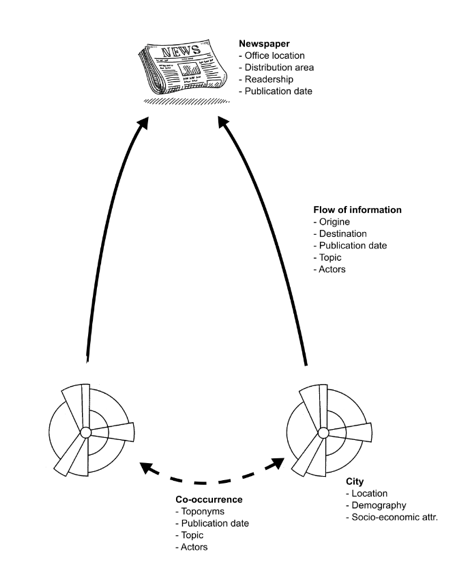
\includegraphics{informationflow}
    \caption{Solid lines represent simple information flows, whereas the dashed line is a complex connection of information. We focus on the part depicted by the dashed line.}
    \label{fig:infoflow}
\end{figure}
\iffalse
\begin{enumerate}
    \item The application could be able to use international names.
    \item A front-end should be build for the UrbanSearch system. This front-end should visualise basic relations and statistics and can be used for presentations or educational purposes
    \item The software should use Delpher to characterise relationships between a region and cities outside that region based on newspapers in those regions, aggregated over the past 50 years. These relationships are either simple or complex information flows. Simple information flows consist of a newspaper located in city i publishing about city j, whereas complex information flows are co-occurrences of cities in an article.
    \item The relations that are extracted from the data by the machine learning algorithm and the relations provided by the CBS have to be visualised in a way that makes it easy to compare the different relations for the end user.
\end{enumerate}
\fi
\subsubsection {Would Like}
"Would like" requirements have been agreed upon to be not important to include within the current time schedule. However, they can be included in future releases.

\begin{enumerate}
    \item The application would be able to show all connections of all places on the map at the same time.
    \item Using data from top-level domains other than \texttt{.nl}.
\end{enumerate}

\subsection{Design Decisions}
To be able to have a fast development cycle and leverage our experience we chose to develop the application using Python. 
We plan to not only test the code we deliver thoroughly, but also to cross-validate the obtained results. The specifics of this validation protocol will be discussed in section \ref{sec:validation_protocol}.
% same as research report, but add section "evaluation strategies"
\section{Frameworks and Tools}

\subsection{Extraction}
\subsubsection{Information Sources}

\paragraph{Common Crawl}
Common Crawl \cite{commoncrawl} is a freely accessible corpus of the pages across the web. Their data is updated and released on a monthly basis. Many researchers have used the data for varying purposes~\cite{smith2013dirt}~\cite{muhleisen2012web}~\cite{singh2012wikilinks}. Since the UrbanSearch project requires us to crawl the web (see section {\color{Red} FIXME}), the corpus is a very suitable candidate for us to work with.

The data of Common Crawl comes in three formats: 
\begin{itemize}
\item[WARC]
\item[WAT]
\item[WET]
\end{itemize}

For extracting data from Common Crawl, many open-source libraries are available. Common Crawls' official website refers to \texttt{cdx-index-client}\footnote{https://github.com/ikreymer/cdx-index-client} as a command line interface to their data. It allows for, among others, specifying which index to use, supports multiple output formats (plain text, \texttt{gzip} or \texttt{JSON}) and can run in parallel.

\paragraph{Eurostat}
{\color{Red} FIXME @Gijs: niet iets zeggen over wat het is?}
We identified Eurostat as a source that is not useful for the problem we're going to solve. Although Eurostat contains a lot of statistics on European cities, there is not enough useful information which contributes to giving more insight into the network connectivity of cities. Therefore, we did not include Eurostat as an information source.
\subsubsection{methods}

\subsection{Filtering and Categorizing}

\subsubsection{Clustering}
\subsubsection{Filtering}
\subsubsection{Machine Learning}
\subsubsection{TF-IDF}
basic idea: 1. using training data to assign values on words - filter meaningless words - assign words with highest value as categories? 2. Do the same on training data for each category (choose a few documents manually per category) and then check for websites for which categories has the highest value.

\subsection{Search Queries}

\subsubsection{Enter Queries}
\subsubsection{Get Results}
\subsubsection{Specifications}

\subsection{Visualisation}
\subsubsection{neo4j?}

\subsubsection{Connection between cities}
\subsubsection{The Strength of these connections}
% Describe how we used the selected tools to actually build the framework
% Also describe the modules we designed, including code snippets and UML stuff
% Make sure to split back-end and front-end here, but discuss how they are linked
\section{Framework Implementation}
%Subsection: Downloading data and parsing indices
%Subsection: Filtering
%Subsection: Classification
%Subsection: Storing data
%Subsection: Front-end
\section{Downloading and Parsing Indices}\label{sec:5-downloading}

As can be seen in figure \ref{fig:overview}, the first step of the process is to download data from Common Crawl. This requires functions that will parse the Common Crawl indices and gather the data that correspond to these indices. 

\begin{figure}[H]
\centering
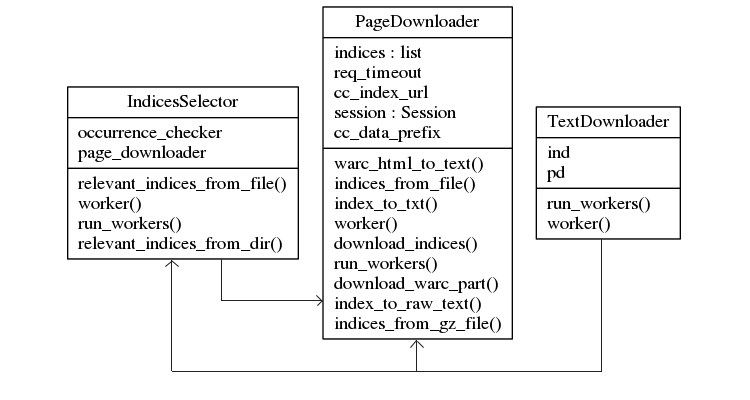
\includegraphics[width=0.8\textwidth]{gathering_class}
\caption{Diagram of downloading and parsing classes}
\label{fig:gathering_class}
\end{figure}

The parsing of indices and downloading of the data depends on the \texttt{IndicesSelector} and \texttt{PageDownloader} class, methods from these classes are called by the \texttt{TextDownloader}, as can be seen in figure \ref{fig:gathering_class}. The classes contain workers, these workers can be run  using the \texttt{run\_workers()} method. This method utilises the Python multiprocessing\footnote{\url{https://docs.python.org/3.5/library/multiprocessing.html}} library to run workers in parallel. Parallelising these workers speeds up the downloading of partial WARC files and parsing of Common Crawl indices.

The first step in parsing the Common Crawl indices is to filter out the indices that have a HTTP Status Code \footnote{\url{https://www.w3.org/Protocols/rfc2616/rfc2616-sec10.html}} other than 200, as only indices with this HTTP Status Code are be useful. 

\begin{lstlisting}[language=Python, caption=Initial implementation, label={lst:initial}]
def _useful_responsecode(self, index):
# Check responsecode of index to determine if it's useful to download
# the part. HTTP 200 is useful, other than 200 will be discarded.
    if index:
        return True if int(index['status']) == 200 else False
    return False

def _clean_indices(self, indices):
    # Removes useless entries with status code other than 200
    for index in indices:
        if not self._useful_responsecode(index):
    indices.remove(index)
\end{lstlisting}

At first, a simple implementation was used as can be seen in listing \ref{lst:initial}. However, removing an element from a Python list is a time complexity of $O(n)$ operation. Since the implementation of \texttt{clean\_indices()} loops over all indices and removes it if it has status code other than 200, this function has a complexity of $O(n^2)$. To improve on this, a regular expression to search the string for the status before parsing to JSON is used. This way, the list will never contain any indices with a HTTP Status Code other than 200. This is because the function will be called in a list-comprehension (see listing \ref{lst:comprehension}). This adjustment resulted in a speedup of about 5.6 times compared to the $O(n^2)$ method.


\begin{lstlisting}[language=Python, caption=Regex solution]
def _useful_str_responsecode(string):
    if string:
        return int(re.search('\"status\": \"(\w+)\",', string)
                   .group(1)) == 200
\end{lstlisting}


\begin{lstlisting}[language=Python, caption=List comprehension creating list of indices, label={lst:comprehension}]
with gzip.GzipFile(filename) as gz_obj:
    # Remove the garbage before {, parse to json and add to list
    indices = [json.loads('{' + x.split('{', 1)[-1]) for x in
               gz_obj.read().decode('utf-8').strip().split('\n')
               if self._useful_str_responsecode(x)]
\end{lstlisting}


While parsing the index, the memory footprint of the indices is also reduced with use of the method from listing \ref{lst:memory}. Parsing every key of the index to JSON means the resulting JSON dictionary is 480 bytes, where the size of the stripped index is 288 bytes. The size of the objects is determined using the Python built-in \texttt{sys.getsizeof()} method. 

\begin{lstlisting}[language=Python, caption=Reducing memory footprint, label={lst:memory}]
def _remove_keys(json_dict):
# Strip all key-value pairs other than digest, length, offset & name
    return {k: v for k, v in json_dict.items()
            if k in ['digest', 'length', 'offset', 'filename']}
\end{lstlisting}

\section{Filtering}
\section{Classification}\label{5-classification}
This section describes how we developed our interface for classifying documents. To provide a complete overview we will first discuss how classifiers are defined. Then we will discuss how classifiers are created or loaded in the system. Finally we will discuss the interface that accepts documents and returns a prediction about the category or categories associated with the supplied document.
\subsection{Scikit Pipelines}
As explained in section \ref{sec:classification-design} we decided to use the Scikit-Learn library for all our classification logic. A key concept of Scikit is the so called \texttt{Pipeline}. A \texttt{Pipeline} in Scikit is an assembly of intermediate transform steps, combined with a final estimator \footnote{\url{http://scikit-learn.org/stable/modules/generated/sklearn.pipeline.Pipeline.html}}. The intermediate transforms transform the input data so that the final estimator performs optimally. In listing \ref{lst:sdgc} we show an example of a \texttt{Pipeline} that we use in the system.\\

\begin{lstlisting}[language=python, caption={SGDC Pipeline}, label={lst:sdgc}]
sgdc = Pipeline([
            ('tfidf', TfidfVectorizer(stop_words=sw.words('dutch'))),
            ('select', SelectPercentile(f_classif)),
            ('clf', SGDClassifier(alpha=0.0001,
                                  average=False,
                                  class_weight=None,
                                  epsilon=0.1,
                                  eta0=0.0,
                                  fit_intercept=True,
                                  l1_ratio=0.15,
                                  learning_rate='optimal',
                                  loss='log',
                                  n_iter=5,
                                  n_jobs=1,
                                  penalty='l2',
                                  power_t=0.5,
                                  random_state=None,
                                  shuffle=True,
                                  verbose=0,
                                  warm_start=False))
        ])
\end{lstlisting}
This \texttt{Pipeline} consists of three parts. The "tfidf"-part transforms a text in to a matrix of words with associated TF-IDF scores (which are calculated first using the training set). The "select"-part selects the best 10 percent of features that are returned by the previous transform, in our case the \texttt{TfidfVectorizer} transform. For this particular \texttt{Pipline} this means that 10 percent of the features with the highest TF-IDF score are returned. Finally, the "clf"-part is the final estimator. For this \texttt{Pipeline} it is a SVM that uses SGD training.\\
After defining the pipeline it can be used to train the classifier. This is done by inputting a set of input with corresponding expected outputs. When the classifier is trained, it can be used to estimate new unseen inputs. 
\subsection{ModelManagers}
To provide an easy way to work with Scikit \texttt{Pipeline}s, we implemented a utility class called \texttt{ModelManager}. The \texttt{ModelManager} is an super class that should be used to implement algorithm specific \texttt{Pipeline}s, while providing easy to use interfaces for loading, saving, training and predicting. Listing \ref{lst:modman} shows a snippet of the \texttt{ModelManager} base class.

\begin{lstlisting}[language=python, caption={ModelManager base class}, label={lst:modman}]
class ModelManager(object):
    """
    ModelManager base class.
    Should only be used to load saved models from disk.
    If a file name is passed this file will be used to load a pickled
    classifier from that location on disk.
    """

    def __init__(self, filename=None):
        super(ModelManager, self).__init__()
        self.x_train = []
        self.y_train = []
        self.x_validate = []
        self.y_validate = []
        self.x_test = []
        self.y_test = []

        self.clf = self.load(filename) if filename else None

    def load(self, filename):
        """
        Load the classifier from the supplied file

        :param filename: the file containing the pickled classifier instance
        :return: a Scikit classifier object
        """
        with open(os.path.join(MODELS_DIRECTORY, filename), 'rb') as f:
            return pickle.load(f)
\end{lstlisting}

The base class can be used to implement specific \texttt{ModelManager}s which define a concrete \texttt{Pipeline} with a final estimator of choice, like the \texttt{MultinomialNB} (Multinomial Naive Bayes) estimator used in listing \ref{lst:mnbmm}.\\

\begin{lstlisting}[language=python, caption={ModelManager using the Multinomial Naive Bayes estimator}, label={lst:mnbmm}]
class MNBModelManager(ModelManager):
    """
    An implementation of the ModelManager base class which uses a Multinomial
    Naive Bayes classifier as its default classifier.
    """

    def __init__(self, filename=None):
        super().__init__(filename)

        if not filename:
            self.clf = Pipeline([
                ('tfidf', TfidfVectorizer(stop_words=sw.words('dutch'))),
                ('anova', SelectPercentile(f_classif)),
                ('clf', MultinomialNB())
            ])
\end{lstlisting}

The \texttt{MNBModelManager} leverages all the load, save, predict and train functionality of the base class.\\
The base class can be used to load saved classifiers from disk. This is done by providing the \texttt{ModelManager} class with a file name on initialisation. If the file is found, the classifier is loaded from disk and ready to be used.

\subsection{ClassifyText Interface}
Most of the time we do not want to be busy with creating and training classifiers, we want to classify documents. To provide an interface that can be used easily to input documents and get back predictions of which category a document belongs to, we implemented the \texttt{ClassifyText} class. The class loads a default classifier that should be available in the correct directory. After the class is initialised, the \texttt{predict} and \texttt{probability\_per\_category} methods can be used to predict categories for given documents.\\

The predict method, which is shown in listing \ref{lst:ct-predict}, takes a document as input and returns a prediction of the category which the inputted document best matches.\\

\begin{lstlisting}[language=python, caption={Predict method of the ClassifyText class}, label={lst:ct-predict}]
def predict(self, text, pre_processor=None):
    """
    Predict the class of the supplied text

    :param :text the text that needs to be classified
    :return: a prediction of the category for the passed text
    """
    if pre_processor:
        text = pre_processor(text)

    return self.mm.predict([text])
\end{lstlisting}



\begin{lstlisting}[language=python, caption={probability\_per\_category method of the ClassifyText class}, label={lst:ct-prob}]
def probability_per_category(self, text, pre_processor=None):
    """
    Predict the class of the supplied text

    :param :text the text that needs to be classified
    :return: a prediction of the category for the passed text
    """
    if pre_processor:
        text = pre_processor(text)

    return dict(zip(self.mm.clf.classes_,
                    self.mm.probabilities([text])[0]))
\end{lstlisting}

\subsection{Overview}
In figure \ref{fig:classify-uml} we give a concise overview of the classification subsystem. The UrbanSearch API is used to classify documents by loading an instance of the \texttt{ClassifyText} class on startup. Furthermore the API offers the possibility to create new (default) classifiers or to modify existing classifiers.\\
The \texttt{ClassifyText} object uses an implementation of the \texttt{ModelManager} class to predict categories of documents.
\begin{figure}[H]
\centering
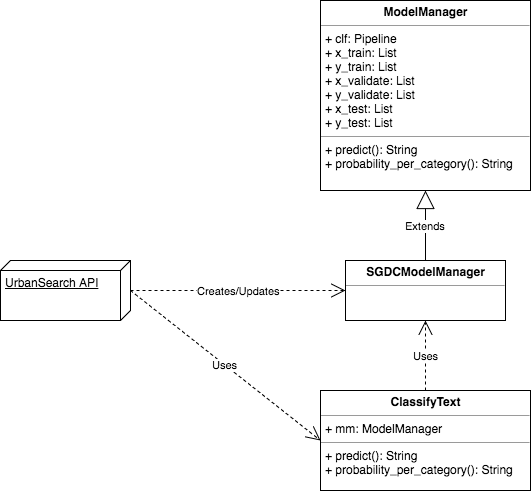
\includegraphics[width=0.6\textwidth]{classify-uml}
\caption{Diagram depicting the interaction between the API and the classification subsystems}
\label{fig:classify-uml}
\end{figure}

\section{Storing the Data}\label{sec: 5-storing}
In this section, we discuss how the filtered documents are stored and how Neo4j was used for storing extracted relations, following the design described in section \ref{sec:storing-design}. We discuss the storage and graph database parts from the overview (see figure \ref{fig:overview}).

\subsection{Storing Filtered Documents}
The documents that pass the filtering stage can be stored for several reasons. For example, the classifier can be retrained and might thus label documents differently. To avoid having to download and process all the pages again, it is useful to store the documents on disk. If the disk is small, it is wise to compress the documents. However, compression is a slow process, so if enough disk space is available, storing the documents uncompressed is more feasible.

In the \texttt{TextDownloader} class, that was already shortly discussed in section \ref{sec:5-downloading}, storage to disk is done without compression in all cases. We did this since this project only involves a relatively small data set, e.g. one that can be stored without the need for compression.

\subsection{Storing Extracted Data}
To be able to interact with the results of the application, it is required to store extracted relations. The implementation of the storage follows the design of section section \ref{sec:storing-data}, using the graph database Neo4j.

\subsubsection{Neo4j Model}
The model used for the graph structure follows the concepts described in section \ref{sec:neo4j-concepts}. It consists of nodes, labels and properties. To distinguish between and to efficiently query for specific (types of) nodes, at least one label is assigned to the node. Below, the labels we used are listed and per label, a description of the nodes they are attached to is given:

\begin{description}
\item[:City] Nodes labelled as \texttt{:City} represent the cities the application uses. These nodes contain multiple properties: name, population, longitude and latitude. Population is used in the visualisation (see section \ref{sec:5-front-end}) for scaling. Longitude and latitude are used to place the cities on a map and were retrieved through the Google Maps Geocoding API\footnote{\url{https://developers.google.com/maps/documentation/geocoding/start?hl=en_US}}. However, this did not work out quite well for duplicate city names. Google picks the coordinates for the city it considers the most important. This was fixed manually. Indeed, this is not a feasible solution, should there be many duplicate city names.
\item[:Index] Nodes with the \texttt{:Index} label represent documents that are found useful. Every document has this label, in addition to the label representing the category they are classified as. The following basic properties belong to these nodes: file name, offset and length. They point to the exact file location where the page can be downloaded from CommonCrawl. Additionally, the nodes contain a probability property per category. These probabilities come from the classifier and are there for validation purposes.
\item[Categories] For each category, a label exists to separate a category from the bulk of documents. This way, documents of a specific category can be matched against. This is particularly useful to count, for example, the documents about "Leisure" (and thus labelled \texttt{:Leisure}), that two cities have in common. Category labels are only applied to nodes that also have the \texttt{:Index} label and thus share the same properties.
\end{description}

The nodes are connected using relations. Cities (\texttt{:City} labelled nodes) occurring in documents (\texttt{:Index} labelled nodes) are connected with a \texttt{:OCCURS\_IN} relation. It is mainly used to find documents in which a pair of cities occurs. For example, the query below matches the documents Rotterdam and Amsterdam have in common and returns the file names:

\begin{lstlisting}[language=cypher, caption={Querying documents containing two cities}, label={lst:query-occ}]
MATCH (:City { name: 'Amsterdam' })-[:OCCURS_IN]->
    (i:Index)
        <-[:OCCURS_IN]-(b:City { name: 'Rotterdam'})
RETURN i.filename
\end{lstlisting}

Intercity relations are the relations between distinct \texttt{:City} labelled nodes and are called \texttt{:RELATES\_TO}. They represent what the client is actually interested in and have a property for every category, containing the score. Additionally, the sum of the individual category scores is kept in a "total" property. The relations are used for exporting, visualisation and interaction. When populating the relations, the count for every category is needed for all city pairs. Cypher, however, has no easy way to count all labels per type. Therefore, the query to achieve the desired counts is slightly more complex than necessary for example in a SQL based query language:

\begin{lstlisting}[language=cypher, caption={Counting distinct labels}, label={lst:query-counts}]
MATCH (:City { name: 'Amsterdam' })-[:OCCURS_IN]->
            (i:Index)
      <-[:OCCURS_IN]-(b:City { name: 'Rotterdam')
WITH DISTINCT LABELS(i) as labels, COUNT(i) AS labelCount
UNWIND labels AS category
RETURN category, SUM(labelCount) AS score
\end{lstlisting}

The query in listing \ref{lst:query-counts} starts with matching all common \texttt{:Index} nodes between Amsterdam and Rotterdam. Then, it collects the labels of the found nodes and counts them.
However, the issue with this is that \texttt{LABELS(node)} returns a list of labels. The counts (\texttt{labelCount}) therefore do not represent individual labels but groups of labels. The lists are therefore expanded using \texttt{UNWIND} and all counts are collected.\\

The full implemented model is given in figure \ref{fig:neo4j-model-full}

\begin{figure}[H]
    \centering
    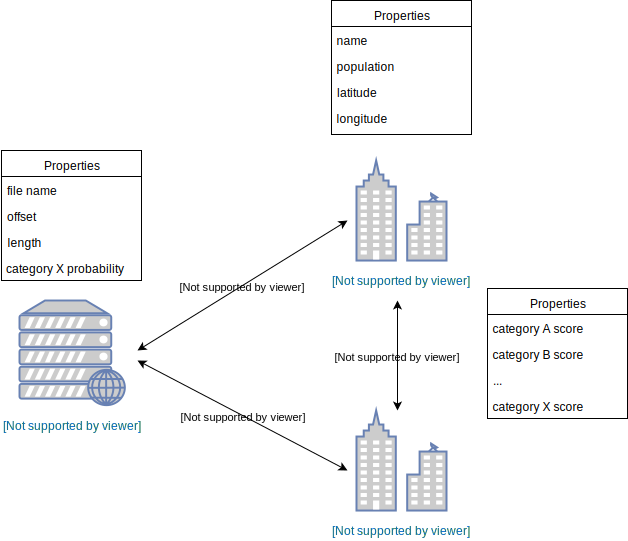
\includegraphics[width=0.6\textwidth]{neo4j-model-full}
    \caption{The Neo4j model as implemented}
    \label{fig:neo4j-model-full}
\end{figure}

During the first tests of the database functions, it appeared that matching and creating was very slow. Checking the query plans (by means of prepending the very useful \texttt{PROFILE} to the queries) gave no hints however. It turned out that we did not use parameterised queries, where we should have. Because of this, Cypher had to recompile, plan and optimise the queries over and over again, which is clearly unnecessary if only the query parameters change. To illustrate the effect of this change, consider the list of cities we used, containing over 1600 cities. Matching all of these in a single transaction by name, without parameterising the query, comes down to repeating the following query for every city:

\begin{lstlisting}[language=cypher, caption={Matching cities without parameterising}, label={lst:query-non-param}]
MATCH (c:City { name: 'Amsterdam' }) RETURN c.name
\end{lstlisting}

The same approach can be used for a parameterised query, where \texttt{\{name\}} is the parameter:
\begin{lstlisting}[language=cypher, caption={Matching cities without parameterising}, label={lst:query-with-param}]
MATCH (c:City { name: {name} }) RETURN c.name
\end{lstlisting}

Even for these 1600 simple matches, the improvements are already significant, as can be seen in table \ref{tbl:param-improvement}.
\begin{table}[H]
\centering
\begin{tabular}{|c|c|}
    \hline
    non-parameterised & 2.84s \\
    parameterised & 0.85s\\
    \hline
\end{tabular}
\caption{Parameterised versus non-parameterised total execution times}
\label{tbl:param-improvement}
\end{table}

Another issue that was encountered during initial testing, is that executing only one query at a time creates and commits a transaction for every query. This is an expensive process. Using the parameterised query from listing \ref{lst:query-with-param} in a single transaction is a 15\% performance gain, as shown in table \ref{tbl:bulk-improvement}. Moreover, it seemed as if performance was fluctuating with a transaction per query. However, we have not benchmarked this.
\begin{table}[H]
\centering
\begin{tabular}{|c|c|}
    \hline
    single transaction & 1.07s \\
    parameterised & 0.85s\\
    \hline
\end{tabular}
\caption{Parameterised versus non-parameterised total execution times}
\label{tbl:bulk-improvement}
\end{table}

As will be explained later in section \ref{sec:main-app}, we use multiprocessing to glue the system together efficiently. However, it turned out that Neo4j did not behave correctly when nodes and relations where matched, updated or created from multiple processes. The number of queries performed did not match the number of results returned. In fact, the numbers diverged about 15\%. However, we currently suspect it is not a platform-wide issue. The server the system runs on successfully inserted 154000 \texttt{:Index} labelled nodes and created all required relations, with the use of multiprocessing. We currently suspect (but cannot verify) the problem is related to the version of Neo4j designed for macOS (which half of the group uses). However, we only discovered this close to the deadline of the project. We therefore decided not to include multiprocessing at all for database communication.

\section{Front-End}
% evaluate the product, and see whether we have at least the minimum viable product
% using the requirements and design goals (possibly in a table)
% make sure to add lots and lots of figures, tables and benchmarks here
% also add SIG stuff and talk about SCRUM
% mention tests
% evaluate the product, and see whether we have at least the minimum viable product
% using the requirements and design goals (possibly in a table)
% make sure to add lots and lots of figures, tables and benchmarks here
% also add SIG stuff and talk about SCRUM
% mention tests
\chapter{Project Evaluation}
\todo{intro}
% evaluate the product, and see whether we have at least the minimum viable product
% using the requirements and design goals (possibly in a table)
% make sure to add lots and lots of figures, tables and benchmarks here
% also add SIG stuff and talk about SCRUM

\todo{Put results in appendix F}
\todo{write conclusion about results}

\section{Fulfilment of Requirements}
In section \ref{sec:reqs} we declared the requirements for our program. Table \ref{requirements_pass/fail} shows which of these requirements passed or failed. \\
\todo{failed must have}
The program works as intended so all must haves passed. \\
There are however two should haves which failed. Finding correct relations proved more time-consuming than expected therefor our algorithm only discerns the top level relations (e.g. trade) and not sub levels (e.g. food trade). Furthermore there are a lot of places with duplicate names, yet no complete lists of these duplicates are available. Therefor it is less easy implementable than first thought. \\
Since other, more important, tasks took longer to implement than intended we did not make implement functionality to use Delpher to characterise relationships. We did add functionality to visualise the data by using a map. \\
As expected the would likes did not pass. It is theoretically possible to show all connections of all places on the map at the same time. However, it would result in a completely filled in map because there is a line for each relation so one would not be able to get any useful information from this.

\todo{more about not mentioned pass/fail, name reqs?}
\todo{Kan die tabel niet beter Requirement:Pass/Fail:Uitleg, en dan voor Must, should etc?}
\begin{table}[h]
\centering
\caption{Requirements pass fail}
\label{requirements_pass/fail}
\begin{tabular}{llllllll}
\begin{tabular}[c]{@{}l@{}}Must \\ Haves\end{tabular} & \begin{tabular}[c]{@{}l@{}}Pass /\\ Fail\end{tabular} & \begin{tabular}[c]{@{}l@{}}Should \\ haves\end{tabular} & \begin{tabular}[c]{@{}l@{}}Pass /\\ Fail\end{tabular} & \begin{tabular}[c]{@{}l@{}}Could \\ Haves\end{tabular} & \begin{tabular}[c]{@{}l@{}}Pass /\\ Fail\end{tabular} & \begin{tabular}[c]{@{}l@{}}Would\\ Haves\end{tabular} & \begin{tabular}[c]{@{}l@{}}Pass /\\ Fail\end{tabular} \\
1                                                     & Pass                                                  & 1                                                       & Fail                                                  & 1                                                      & Fail                                                  & 1                                                     & \todo{Pass?}                                                      \\
2                                                     & Fail                                                  & 2                                                       & Pass                                                  & 2                                                      & Pass                                                  & 2                                                     & Fail                                                       \\
3                                                     & Pass                                                  & 3                                                       & Pass                                                  &                                                        &                                                       & 3                                                     &                                                       \\
4                                                     & Pass                                                  & 4                                                       & Fail                                                  &                                                        &                                                       &                                                       &                                                       \\
5                                                     & Pass                                                  &                                                         &                                                       &                                                        &                                                       &                                                       &                                                      
\end{tabular}
\end{table}

\section{Process}

\subsection{Collaboration Between the Team Members}
The collaboration between the team members went well. The team members worked in a room in the faculty of architecture from 9-5 each day. Three of the four team members knew each other already. The work was divided even over the team members. 

\subsection{Collaboration Between the Team Members and the TU Delft Coach}
Each week 9:30 on Monday the team members had a meeting with the TU Delft coach. In the beginning there were some communication issues between the team and the coach but as the process went on communication became better.
\todo{Claudia absent twice}

\subsection{Collaboration Between the Team Members and the Client}
The collaboration between the team members and the client was good as well. 
Weekly meetings helped the team members making the product as good as possible to the clients wishes. 
% evaluation protocol results
% describe issues faced during implementation, as well as issues that are still 
% open. Main thing here is to discuss the Neo4j python driver with multiprocessing,
% which we could not get to work. Also mention the state of the document 
% classification
% DONT FORGET a subsection on ethical issues!
\chapter{Discussion}
% See http://libguides.usc.edu/writingguide/discussion for how to write a discussion

This section is divided into three parts. First we will discuss the influence of the research questions. Next we will mention issues we faced and which still remain. The last part of this section is dedicated to the ethical questions this project may involve.

\section{Discussing the research question answers something} \todo{better title}

\section{Issues Faced During Development}
\todo{memory problems}
    
\todo{multiprocessing}
\todo{text encoding}
\todo{python neo4j driver}


\section{Open Issues}
\todo{Discuss choice to filter "Amsterdammers", future version might include this}
\todo{exporting data}
\todo{uneven amount of documents/class}
\todo{language}
\todo{processing time}
\todo{neo4j problems}
\todo{more....}

% describe issues faced during implementation, as well as issues that are still 
% open. Main thing here is to discuss the Neo4j python driver with multiprocessing,
% which we could not get to work. Also mention the state of the document 
% classification
\section{Classification}
% Describe issues faced during implementation/development
%Discuss open issues 

\section{Ethics}
In this section some of the ethical issues with respect to the developed product are discussed. 

\subsection{Storage}
%One ethical issue is due to the storing of data. Since we store random web pages we do not know whether or not these pages may contain private or copyrighted data. For instance news articles could be downloaded and stored whilst this could violate the copyright issues. For most free news sites this is not a problem but this especially becomes a problem when using Delpher as a data source. Therefor if this source is added it must also be ensured that the data is stored in a safe way.

\subsection{Impact of Found Relations}
%Another issue that may occur is the influence this kind of research may have. If there is indeed a correlation between the results of our program and the economic growth of cities this may influence the behaviour of investors, companies and cities. Investors may look at the data and decide to invest in companies from more growing cities. Companies may use this data to decide where to build their new offices. And cities may change their policies based on the results. In future executions of our system it may also occur that data is being manipulated. Involved parties which put extra data online containing the names of cities they want to have a better result for. Whilst these issues may occur, we do not suspect our system to have a large enough impact to cause this. It may rather be a step towards these effects. Over time the effects will become clearer and they should be taken into account when continuing research in this field.

% Make recommendations for future version, for extending the back-end and front-end
% Try to mention the requirements here
\section{recommendation}
% Start with "In the past few months we blah" and shortly mention the chapters
% Mention the project goal and how well it is met, without duplicating the 
% evaluation chapter
\chapter{Conclusion}

\todo{ Start with "In the past few months we blah" and shortly mention the chapters
 Mention the project goal and how well it is met, without duplicating the 
 evaluation chapter}

\section{related work}
First, we discussed related work. We saw that there are currently two methods for analysing the relations between cities. Manually analysing search engine data is very slow and requires a lot of man-hours and looking at the different locations where businesses are located is only interesting for the economic relation and still misses a lot of data.
\\

\section{related work}
Second, we identified the requirements for a solution to the problem and discuss issues that might arise. The used the MoSCoW model to describe the importance of the different requirements. The most import must haves we found are being able to input place names, displaying a map with the connection data and being able to extract this data.
\\

\section{Requirement analysis}
Third, we developed a methodology for a framework that satisfies the requirements and tackles the issues. We decided to start by using data from Common Crawl, although we might later extend this to other data sources such as Delpher. After selecting relevant data (data which contains 2 or more city names) we store the data with Neo4j. We then use clustering and classifying machine learning to group the data. First we use this on all data to get the general groups (e.g. economy, health-care, immigration) and then we use this on the data per pair of cities to see what the important connection types for each city are. Then we link these connections to the general groups ('fish' might relate to economy.. etc). To visualise this data we use the graph Neo4j provides.

\section{Framework-and-tools}


\bibliography{references}{}

\appendix
\chapter{Better Code Hub Guidelines}\label{bch_guidelines}
\addtocontents{toc}{\protect\setcounter{tocdepth}{0}}

Better Code Hub \cite{better_code_hub} checks our code according to ten guidelines:
\begin{enumerate}
    \item \textbf {Write short units of code} \\
    Units of code should be no longer than 15 lines.
    \item \textbf {Write simple units of code} \\
    Separate units of code should contain no more than 4 branch points (if, for, while, etc)
    \item \textbf{Write code once} \\
    Shared code should be extracted, either to a new unit or to a super class
    \item \textbf{Keep unit interfaces small} \\
    The number of parameters per unit of code should be no more than four.
    \item \textbf{Separate concerns in modules} \\
    Identify and extract responsibilities of large modules to separate modules and hide implementation details behind interfaces.
    \item \textbf{Couple architecture components loosely} \\
    minimizing the amount of interface code (e.g. by using 'abstract factory' design pattern)
    \item \textbf{Keep architecture components balanced} \\
    Organize code in such a way that the number of components is between 2 and 12, and ensure the components are of approximately equal size (keep component size uniformity less than 0.71).
    \item \textbf{Keep your codebase small} \\
    Refactor existing code to achieve the same functionality using less volume, and prefer libraries and frameworks over "homegrown" implementations of standard functionality.
    \item \textbf{Automate tests} \\
    Add tests for existing code every time you change it.
    \item \textbf{Write clean code}\\
    Remove useless comments, commented code blocks, and dead code. Refactor poorly handled exceptions, magic constants, and poorly named units or variables.  
\end{enumerate}
\newpage
\chapter{Sig Feedback}\label{sig_fb}
\section{week 5}
[Analyse]

De code van het systeem scoort 4 sterren op ons onderhoudbaarheidsmodel, wat betekent dat de code bovengemiddeld onderhoudbaar is. De hoogste score is niet behaald door een lagere score voor Unit Complexity.

Voor Unit Complexity wordt er gekeken naar het percentage code dat bovengemiddeld complex is. Het opsplitsen van dit soort methodes in kleinere stukken zorgt ervoor dat elk onderdeel makkelijker te begrijpen, makkelijker te testen is en daardoor eenvoudiger te onderhouden wordt.

Omdat jullie qua score al vrij hoog zitten gaat het hier voornamelijk om kleine refactorings. Methodes als IndicesSelector.run\_workers en CoOccurrenceChecker.\_calculate\_occurrences zou je nog iets verder kunnen opsplitsen in functionele gebieden.

De aanwezigheid van test-code is in ieder geval veelbelovend, hopelijk zal het volume van de test-code ook groeien op het moment dat er nieuwe functionaliteit toegevoegd wordt.

Over het algemeen scoort de code bovengemiddeld, hopelijk lukt het om dit niveau te behouden tijdens de rest van de ontwikkelfase.

\section{week 9}
\newpage
\section{User manual}
\chapter{Developers Manual}
\chapter{Used Libararies}
\chapter{Validation and Verification results}\ref{app:val_ver_results}

To ensure code quality in our project we used several methods. The results from SIG \cite{sig}, a tool to ensure code quality and maintainability, are discussed and the testing is discussed.


\section{Testing the Application}

\subsection{Unit Tests}

\subsection{Integration Tests}

\subsection{System Tests}

\subsection{Acceptance Tests}

\section{SIG}
SIG, Software Improvement Group, gives detailed insight needed to achieve better code quality and maintainability. SIG rates the code on a five star scale based on nine different values concerning code quality. Before submitting code to SIG we used BetterCodeHub\cite{better_code_hub} to check for possible faults in our code. BetterCodeHub does partly what SIG also does, but it is done online instead and can be done on every moment. Code was submitted to SIG on week 5 and week 9 of the project. Since the final report is due to the same date as the second submission for SIG review, the second review will not be included in this report. Instead we will show the final results from BetterCodeHub for week 9. Exact feedback can be found in appendix \ref{sig_fb}.


\subsection{week 5}
The first feedback from SIG was in the fifth week of development. Before uploading on BetterCodeHub our code passed all checks. For SIG it had a score from four out of five stars which means our code is above average maintainable. The last star was missed because the code is above average complex. This means that some of the functionality of some methods should be split into separate methods.
\todo{fixed this?}

\textbf{week 9} \\

\section{evaluating the classification}

\subsection{Accuracy}

\subsection{Confusion Matrix}

\subsection{Precision, Recall, F1 and UAC}

\section{Evaluation of relation scores}




\end{document}
